\section{Textbook Materials}

\subsection{Writing about Numbers}

\begin{frame}
    \frametitle{Outline}
    \tableofcontents[currentsection, currentsubsection]
\end{frame}
\begin{frame}
    \frametitle{Seven Basic Principles}
     \begin{enumerate}
         \item Set the context 
         \item Choose effective examples and analogies
         \item Choose vocabulary to suit your readers
         \item Decide whether to present \#s in text, tables, or figures
         \item Report and interpret \#s in the text
         \item Specify the direction \emph{and} size of an association between variables
         \item For many \#s, summarize overall pattern 
     \end{enumerate}
\end{frame}

\begin{frame}
    \frametitle{WMA Problem 2.5a \& 2.6a}
        \begin{verse}
            The Williams family's income of \$25,000 falls below 185\% of the 
            \href{http://aspe.hhs.gov/poverty/12poverty.shtml}{Federal Poverty
            Threshold} for a family of four, qualifying them
            for food stamps. 
        \end{verse}
        \vskip0.3in
\begin{description}
    \item[Problem 2.5a] {Identify terms that need to be defined or restated
        for a nontechnical audience}
    \item[Problem 2.6a] Rewrite the sentences in the previous questions for an
        audience with a fifth-grade education.  Convey the main point,
        not the calculation or the jargon. 
    \item[FYI] \href{http://www.bloomberg.com/video/how-the-rich-get-richer-and-the-poor-poorer-kfuILNN9SoaQXLd5cVBwPQ.html}{Off-the-chart}
\end{description}
        
\end{frame}

\begin{frame}
    \frametitle{WMA Problem 2.8a}
    Rewrite each of these sentences to specify the direction and magnitude of
    the association:
    \vskip0.1in
    \begin{center}
    \begin{verse}
        In the United States, race is correlated with income. 
    \end{verse}
    \end{center}
    \begin{table}
        \centering
        \caption{\textbf{Median income by race and Hispanic origin, United States, 1999}}
        \label{tab:WMAex2x8}
        \begin{tabular}{lc}
        Race/Hispanic origin & Median Income \\
        \hline 
        White   & \$42,504 \\
        Black   & \$27,910 \\ 
        Asian/Pacific Islander   & \$51,205 \\ 
        Hispanic (can be of any race) & \$30,735 \\
        \hline
        \end{tabular}
    \end{table}
\end{frame}

\begin{frame}
    \frametitle{WMA Problem 2.9}
    Use the GEE approach to describe the patterns in the figure below,
    including an introductory sentence about the purpose of the chart 
    before summarizing the patterns. 
    \begin{figure}
        \begin{center}
            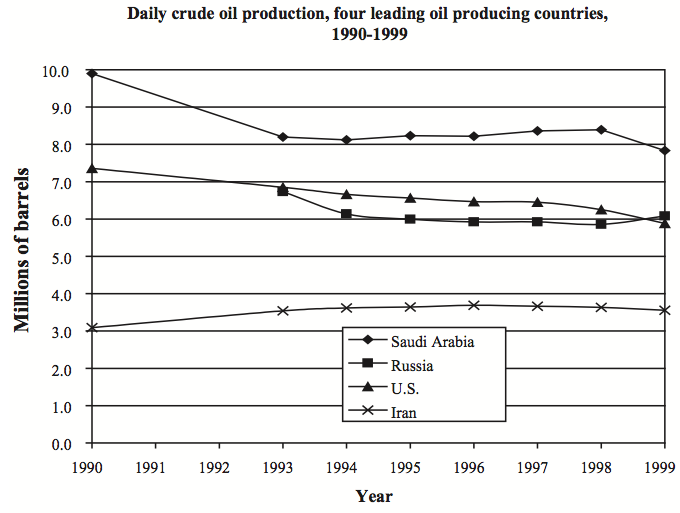
\includegraphics[width=0.6\textwidth]{images/WMAex2x9.png}
        \end{center}
    \end{figure}
\end{frame}

\subsection{Math. Modeling}


\begin{frame}
    \frametitle{Outline}
    \tableofcontents[currentsection, currentsubsection]
\end{frame}

\begin{frame}
    \frametitle{Models and Reality: ``Disclaimer''}
    \begin{verse}
        Here we are concerned exclusively with mathematical models, that is,
        models that mimic reality by using the language of mathematics.
        Whenever we use ``model'' without a modifier, we mean ``mathematical
        model.''
    \end{verse}
\end{frame}

\begin{frame}
    \frametitle{Models and Reality}
    \begin{verse}
    What makes Mathematical models useful? 
    If we ``speak in mathematics,'', 
    \begin{itemize}
        \item We must formulate our ideas precisely and so are less likely to
            let implicit assumptions slip by,
        \item We have a concise ``language'' which encourages manipulation,
        \item We have a large number of potential theorems available,
        \item We have high speed computers available for carrying out calculations.
    \end{itemize}
    \end{verse}
\end{frame}

\begin{frame}
    \frametitle{Properties of Models}
    \begin{verse}
        A mathematical model is an abstract, simplified, mathematical
        construct related to a part of reality and created for a particular
        purpose.
    \end{verse} 
    \begin{verse} 
        Since a dozen different people are likely to come up with a
        dozen different definitions, don't take this one too seriously;
    \end{verse}
    \begin{verse}
        rather, think of it as a crude starting point around which to build
        your own understanding of mathematical modeling.
    \end{verse}
\end{frame}

\begin{frame}
    \frametitle{Properties of Models}
    \begin{verse}
    As far as a model is concerned, the world can be divided into three parts:
    \begin{enumerate}
        \item Things whose effects are neglected,
        \item Things that affect the model but whose behavior the model is not
            designed to study,
        \item Things the model is designed to study the behavior of. 
    \end{enumerate}
\end{verse}
\end{frame}

\begin{frame}
    \frametitle{Building a Model: ``Disclaimer''}
    \begin{verse}
        Model building involves imagination and skill. Giving rules for doing
        it is like listing rules for being an artist; at best this provides a
        framework around which to build skills and develop imagination. 
    \end{verse} 
    \begin{verse}
        It may
        be impossible to teach imagination. I won't try, but I hope this book
        provides an opportunity for your skills and imagination to grow. With
        these warnings, I present an outline of the modeling process.
    \end{verse}
\end{frame}


\begin{frame}
    \frametitle{Building a Model}
    \begin{verse}
        With these warnings, I present an outline of the modeling process.
    \begin{description}
        \item[1.] {Formulate a problem}
        \item[2.] {Outline the model}
        \item[3.] {Is it Useful?}
        \item[3.] {Test the model}
    \end{description}
    \end{verse}
\end{frame}

\begin{frame}
    \frametitle{Building a Model}
    \begin{verse}
        Some models may require no data. If a model makes the same prediction
        regardless of the data, we are not getting something for nothing because
        this prediction is based on the assumptions of the model. 
    \end{verse}
   
    \begin{verse}
        To some extent,
        the distinction between data and assumptions is artificial. In an extreme
        case, a model may be so specialized that its data are all built into the
        assumptions.
    \end{verse}
\end{frame}

\begin{frame}
    \frametitle{Building a Model}
    \begin{verse}
        The manager of a large commercial printing company 
        asks your advice on how many salespeople to employ.  
    \end{verse}
    \begin{verse}
        Qualitatively, more salespeople will increase sales overhead,
        while fewer salespeople may mean losing potential customers. 
    \end{verse}
    \begin{verse}
       Thus there should be some optimum number.
    \end{verse}
    
\end{frame}


\begin{frame}
    \frametitle{IMM Problem: ``Disclaimer''}
    \begin{verse}
        Some of the problems in this book lead you step by step through the
        development of a model and thus resemble the mathematics problems you have
        seen in other courses; 
    \end{verse} 
    \begin{verse} 
        however, many problems are closer to real life:
        They are vaguely stated, have multiple answers (models), or are open
        ended. 
    \end{verse}
    \begin{verse}
        I strongly recommend working in small groups on the problems to
        bring out various ideas and evaluate them critically.
    \end{verse}
\end{frame}

\begin{frame}
    \frametitle{IMM Problem 1.1}
    Suppose people enter the elevators in a skyscraper at random during the
    morning rush. The result will be several elevators stopping on each floor
    to discharge one or two passengers each. 
    \vskip0.1in
    \begin{itemize}
        \item Discuss schemes for improving the situation. 
        \item How could improvement be measured? 
        \item How could you model the situation to decide what scheme to adopt?
    \end{itemize}
\end{frame}

\begin{frame}
    \frametitle{IMM Problem 1.6}
    Unless you have been extremely lucky, you have had a large class in a
    poorly designed lecture hall. 
    
    \vskip0.25in
    \begin{description}
        \item[(a)] What are some criteria to be considered
    in designing a large lecture hall? 
    \end{description}
\end{frame}
    
\begin{frame}
    \frametitle{IMM Problem 1.6}
    Unless you have been extremely lucky, you have had a large class in a
    poorly designed lecture hall. 
    \vskip0.15in
    \begin{description}
        \item[(b)] One criterion is legibility of material written on the boards. 
        \begin{itemize}
            \item Construct a model of legibility as a function of 
                \begin{itemize}
                    \item  \emph{the distance} your seat is from the board 
                    \item \emph{the angle} at which you look at the board 
                \end{itemize}
            \item What will the curves of constant legibility look like on a
                floor plan?
            \item How can you test this prediction? Try it. 
            \item Does this suggest shaping the back of the hall differently
                than is usually done? How?
        \end{itemize}    
    \end{description}
    \vfill
\end{frame}
     
\begin{frame}
    \frametitle{IMM Problem 1.6}
    Unless you have been extremely lucky, you have had a large class in a
    poorly designed lecture hall. 
    
    \vskip0.25in
    \begin{description}
        \item[(c)] Can mathematical modeling help with any other criteria
    besides the one mentioned in (b)? Try to pick a criterion from among these
    possibilities and develop a model for it.
    \end{description}
\end{frame}
     
\begin{frame}
    \frametitle{Models and Reality}
    \begin{verse}
        The ultimate test of a model is how well it performs when 
        it is applied to the problem it was designed to handle.
    \end{verse}
    \vskip0.5in
    \begin{verse}
       A model is used, it may lead to incorrect predictions. The model is
       often modified, frequently discarded, and sometimes used anyway because
       it is better than nothing. This is the way science develops.  
    \end{verse}
\end{frame}




\section{Course Project}

\begin{frame}
    \frametitle{Outline}
    \tableofcontents[currentsection, currentsubsection]
\end{frame}


\begin{frame}[fragile]
    \frametitle{Mission Impossible?: an analogy}
    \begin{figure}
        \caption{Mission Impossible Season 2 Episode (00:00 -- 06:25)}
    \begin{center}
    \href{http://movies.netflix.com/WiPlayer?movieid=70157337&trkid=4431095&pt_request_id=a8a7108c-c068-4d22-b649-0b7095279045-1882594&pt_rank=4&pt_row=-1&pt_location=WATCHNOW#MovieId=70157337&EpisodeMovieId=70156671}{
            
\includegraphics[width=0.8\textwidth]{images/IMFproblemstatement.png}
    }
    \end{center}
    \end{figure}
\end{frame}

\begin{frame}
    \frametitle{Project in Industry: Frequently Recurring Elements}
    A stylized timeline:
    \vspace{7pt}
             \begin{enumerate}
                 \item Work Statement,
                 \item Midterm Presentation,
                 \item Progress Report,
                 \item Final Presentation,
                 \item Final Report.
             \end{enumerate}
    \begin{center}
        \href{http://www.ipam.ucla.edu/programs/rips2011/}{
        
\includegraphics[width=0.5\textwidth]{images/ipam}}        
    \end{center}
\end{frame}

\subsection{Work Statement}

\begin{frame}
    \frametitle{Outline}
    \tableofcontents[currentsection, currentsubsection]
\end{frame}

\begin{frame}
    \frametitle{What is Work Statement}
This is the written proposal and definition of the project and constitutes the
team's ``contract'' with the sponsor. It should be approximately 2-5 pages
long.  It sets forth the nature of the project, the specific
objectives of the project, the results expected, and the ``deliverables'' for
the project. The scope of the project must be within the timetable for the
program and that the deliverables are reasonable and appropriate; given the
nature of research, it should not include promises that the team cannot be
certain to achieve. It is ultimately given to the sponsor for review and
signature.
\end{frame}


\begin{frame}
    \frametitle{Template 1}
    \begin{enumerate}
        \item Abstract
        \item Background
        \item Problem description
        \item Approach (``time permitting'' clause for some work)
        \item Schedule (dates for completing milestones and tasks and for
            deliverables)
        \item Milestones (major checkpoints your team will use to stay on
            track)
        \item Deliverables (specific work products you will deliver to the
            sponsor)
    \end{enumerate}
\end{frame}

\begin{frame}
    \frametitle{Templates 2}
    \begin{enumerate}
        \item Introduction
        \item Problem background
        \item Mathematical background
        \item Computing background 
        \item Possible solutions and project objectives
        \item Deliverables (``time permitting'' clause for some work)
        \item Timeline
    \end{enumerate}
\end{frame}

\begin{frame}
    \frametitle{Template 3}
    \begin{enumerate}
        \item Project background
        \item Goals (major direction you see the work aimed at, not
            necessarily what you bid to do)
        \item Proposed mathematical approach
        \item Objectives (specific aims of your project, and schedule of
            results you expect to achieve)
        \item Optional objectives 
        \item Deliverables
        \item Milestones
        \item Work flowchart
        \item Schedule
    \end{enumerate}
\end{frame}

\begin{frame}
    \frametitle{Template 4}
    \begin{enumerate}
        \item Abstract
        \item Problem background
        \item Problem description
        \item Approach 
        \item Deliverables
        \item Timetable
        \item Team members
    \end{enumerate}
\end{frame}

\begin{frame}
    \frametitle{Work Statement}
    \begin{block}
        {In the initial segment (``Abstract'', ``Introduction'', ``Background'')}
        \begin{itemize}
            \item Brief description of the company
            \item Major product lines(s)
            \item A brief (abstract) description of the project
        \end{itemize}
    \end{block}
\end{frame}

\begin{frame}
    \frametitle{Work Statement}
    \begin{block}
        {Throughout}
        \begin{itemize}
            \item Spell out terminology -- avoid undefined jargon or acronym
            \item When options must be resolved, give dates by which they must
                be resolved
            \item Give modest objectives, not boastful ones
        \end{itemize}
    \end{block}
\end{frame}

\begin{frame}
    \frametitle{Work Statement}
    \begin{block}
        {List of deliverables should include}
        \begin{itemize}
            \item Site visits (to be arranged)
            \item Midterm oral presentation
            \item Midterm report
            \item Final presentation
            \item Final report
            \item Software (if appropriate) 
                \begin{itemize}
                    \item Specify sponsor-approved OS, platform
                    \item Documentations
                \end{itemize}
        \end{itemize}
    \end{block}
\end{frame}

\begin{frame}[allowframebreaks]
    \frametitle{Glossary}
    \begin{block}
        {GOAL} The overall, long range, end result that your research is aimed at, what
you are trying to achieve ultimately. Stating a goal does not mean you believe
you will get there this time around. It is the grand view towards which you
strive. The goal of AIDS research is to find a cure for AIDS.
\end{block}
\end{frame}

\begin{frame}
    \frametitle{Glossary}
    \begin{block}
        {OBJECTIVES} The specific things you will try to achieve in your project, the
immediate targets of your research. Your objectives spell out how you have
parsed the problem of heading towards the goal into smaller pieces that you
will work on. The objectives set practical limits on your work. They point to
where the project can reasonably expect to wind up. It should be clear that
the objectives fit into and work towards the long-range goal.
\end{block}
\end{frame}

\begin{frame}
    \frametitle{Glossary}
\begin{block}
        {TASKS} These are the specific things you will do in order to achieve your
objectives. The tasks drive your determination of what skills and other
resources (such as data, software, hardware, written materials, work
environment) will be needed for your project. If among the resources needed
are ones that must be supplied by the sponsor, then you will need to specify
these items in your Work Statement.
\end{block}
    
\end{frame}


\begin{frame}
    \frametitle{Glossary}
\begin{block}
        {DELIVERABLES} The things you promise to deliver to the sponsor. For a 
project, these include a mid-term and final report, a mid-term presentation
and a final presentation on Projects Day. They may also include site visits to
the sponsor (usually one near the beginning of the project to get acquainted
with the sponsor, and one after Projects Day to present the work at the
sponsor's location), software, perhaps hardware in some cases, written results
of literature searches, white papers (i.e., written background information on
such things as plans, methods or concepts prepared for internal use), etc.
These additional items are to be decided by you in consultation with your
sponsor’s mentor.
\end{block}
    
\end{frame}

\begin{frame}
    \frametitle{Glossary}
\begin{block}
        {MILESTONES} A list of specific accomplishments that you may use to mark
progress and maintain pace and coordination within your project. They are used
to help your team stay on track and to determine the success of a chosen line
of attack on your problem. Milestones may or may not be included in your Work
Statement, but you should definitely think these through for your own use as
you plan your project and Work Statement. They are check-points for you (and
for your sponsor, if they are included in the Work Statement), not necessarily
deliverables. You may want to specify major milestones in your Work Statements
to indicate what you would do if your research leads 
to the conclusion that some objective cannot be accomplished. For example, "if
by such a date we have found it impossible to achieve X, then we will begin
Y." Research is exploration of the unknown, so you may encounter an
intractable obstacle and need to work around it. You can't know everything
ahead of time. Give some thought to this and try to allow for milestones by
which you can judge where you are and what you need to do to proceed
effectively in the event you don't meet a milestone.
\end{block}
    
\end{frame}

\begin{frame}
    \frametitle{Glossary}
\begin{block}
        {SCHEDULE} This specifies when you will finish major parts of your research and
provides a timetable for completion of deliverables. Internally, you should
maintain as fine-grained a schedule as you need to keep your team coordinated
and on track, but in your Work Statement it is best to make the schedule and
list of deliverables as modest as the sponsor will allow.
\end{block}
    
\end{frame}
